%\documentclass[english]{uzhpub}
\documentclass[12pt]{article}
\usepackage[T1]{fontenc}
\usepackage[latin9]{inputenc}
\usepackage{listings}
\usepackage{color}
\usepackage{longtable}
\usepackage{url}
\usepackage{graphicx}

\begin{document}



%% Titelei
\title{Master Project: Clustermeister}

%\subtitle{Report}

\author{Daniel Spicar, Thomas Ritter}

\date{\today}

\maketitle

\definecolor{lbcolor}{rgb}{0.9,0.9,0.9}
\definecolor{white}{rgb}{1.0,1.0,1.0}

\section{Motivation}

Programming distributed systems poses a number of challenges for a developer. One of these challenges is to request, configure and start a distributed computing infrastructure. This is the problem of provisioning. Another challenge is to package, deploy and run code on the distributed computing infrastructure. This is the problem of deployment and execution. Clustermeister has been made to support Java/Scala developers in tackling this challenge by providing dynamic provisioning and deployment in cloud and cluster computation environments.

Dynamic provisioning means that with Clustermeister a developer can set up a distributed computation environment, and then alter it at any time during a session. In Clustermeister terminology a developer can add and remove nodes and shut the environment down again. A node is an addressable unit that can execute code. Clustermeister abstracts the underlying specifics of the computation environment from the user. This way multiple environment can be supported and the user does not have to maintain various tools and scripts and interact with different APIs.

Dynamic deployment means that Clustermeister can deploy new and changed code to nodes without the need to interact with the distributed computation environment manually. This means a developer can just run changed code and does not need to worry about updating and restarting code deployments in the distributed environment. This can save a lot time and hassle when developing a distributed system.

Provisioning and deployment are tasks that interact with distributed computation environments and this is handled transparently to the user by the Clustermeister Provisioning module. Code execution on the other hand must interact closely with user code. For this purpose the Clustermeister API forms a bridge between the infrastructure provided by Clustermeister and the user code. The API offers various methods for code execution. Some allow to address specific nodes, others will distribute tasks to available nodes transparently.

The aim of the project is to support developers by letting them concentrate on their code and solve infrastructure challenges reliably and with minimal configuration.

\subsection*{Clustermeister provides:}
\begin{itemize}
\item Dynamic distributed computation infrastructure provisioning.
\item Dynamic class-loading allowing for client code execution without manual re-deployment.
\item Easy deployment of dependencies using Apache Maven dependency resolution.
\item Parallel and distributed code execution via a Java ExecutorService interface or a native inferface.
\item Addressable nodes for code execution on specific nodes.
\item Provisioning of Amazon Web Services Elastic Compute Cloud (EC2) and TORQUE (PBS) infrastructure.
\end{itemize}

\section{Evaluation of Third-Party Libraries}

Java was chosen as the platform for Clustermeister, because it was known that Clustermeister will be used by Scala clients, so the JVM was a logical decision. Another goal was to licence Clustermeister under the Apache Licence, version 2.0. These were the two most important constraints while searching for suitable libraries.

The goal for Clustermeister was not to re-implement a node runtime based on Java, so instead existing libraries were evaluated that would help to run code on remote JVMs. Ideally, this runtime should provide a means of dynamically loading libraries and classes from the machine that is issuing the computation task.

There are a few libraries that would fit the needs. We selected three libraries to evaluate. These are 
GridGain\footnote{http://www.gridgain.com/}, 
Hazelcast\footnote{http://www.hazelcast.com/} and 
JPPF\footnote{http://jppf.org/}. In the following, these libraries and their characteristics are discussed.

\paragraph{GridGain} GridGain was very easy to set up, has a pleasant API and worked out of the box. It is able to remotely load libraries and classes without additional configuration. However, newer versions of GridGain are licenced under the GPL. Further, there was no obvious way to configure GridGain programmatically. Because of these reasons, GridGain was ruled out.

\paragraph{Hazelcast} Hazelcast was a good fit at first sight, due to its nice API. However, it lacked features that were needed for Clustermeister, i.e. remote deployment of libraries and classes and provisioning capabilities. Hazelcast is generally a low-level solution and it would have required more implementation effort to integrate it into Clustermeister.

\paragraph{JPPF} JPPF was a good fit for the requirements. It is licenced under the Apache Licence and is being actively developed. Further, there is good community support and it fits the needs for Clustermeister. Therefore, JPPF was chosen to build the basic infrastructure.

\section{Architecture and Specification}
\label{architecture}

In this section, Clustermeister's high-level architecture is characterized. First, Clustermeister terminology is introduced. Second, the most important building blocks and modules are presented. At the end of this section, the Clustermeister topology is explained with an example set-up.

\subsection{Terminology}

\begin{description}
\item[Clustermeister Node] A node can be interpreted as a JVM that executes code. Nodes are running on local or remote Clustermeister instances. A single instance can host several nodes.
\item[Clustermeister Instance] An instance is a physical or virtual machine generally running in a cluster or a cloud computation service such as Amazon EC2.
\end{description}

\subsection{Use Cases}

\subsubsection*{Abstract Use Case}
This abstract use case that has been compiled from the project definition and discussion among the developers and the project leadership. It aims to demonstrate how Clustermeister can be used in a development workflow. The use case applies to Java and Scala developers.

\begin{enumerate}
\item \label{uc:start}The developer begins a programming session.
\item The developer starts Clustermeister locally from the command line.
\item \label{uc:alloc}Using the terminal where Clustermeister is running, the developer allocates five Clustermeister nodes in a distributed computation infrastructure.
\item \label{uc:prog}The developer programs a parallel algorithm and uses the Clustermeister API in the source code to submit parallel tasks to the Clustermeister nodes requested in step \ref{uc:alloc}.
\item The developer compiles the code and executes it. The result is not as expected.
\item The developer corrects a bug in the source code, re-compiles it and executes it again. This time the result is correct.
\item The developer wants to speed up the computation. He opens the terminal where Clustermeister is running and requests another five Clustermeister nodes.
\item The developer executes his program again, without re-compilation. This time the result has been computed faster.
\item The developer is satisfied with the result and de-allocates all Clustermeister nodes using the terminal where Clustermeister is running.
\item The programming session ends.
\end{enumerate}

\subsubsection*{Specific Use Cases}
There are many specific use cases that can be derived from this abstract use case. Here are examples of specific variations that will be supported:

\begin{description}
\item[Step \ref{uc:start}.1] The developer wants to execute some code in a distributed manner, not planning to do any development.
\item[Step \ref{uc:alloc}.1] The developer allocates five nodes in the Amazon Web Services Elastic Compute Cloud (EC2).
\item[Step \ref{uc:alloc}.2] The developer allocates five nodes in the TORQUE Cluster provided at the department of informatics in the University of Zurich.
\item[Step \ref{uc:prog}.1] The developer programs a distributed AKKA\footnote{http://akka.io/} actor system. The Clustermeister API allows to iterate through available nodes and bootstrap an actor system by submitting actors to the nodes for execution.
\end{description}

\subsection{Specification}
In the project definition the following requirements relevant for the architecture have been identified:

\begin{enumerate}
\item A method of querying the state of the provisioned infrastructure (Clustermeister nodes) must be available in Clustermeister.
\item A method of adding and removing nodes to or from the provisioned infrastructure must be available in Clustermeister.
\item Clustermeister must offer an API that can be used from Java and Scala and enables user code to interact with Clustermeister nodes. The API must offer:
\begin{enumerate}
\item Access to a Java collection describing all available nodes.
\item Nodes offer a method to submit code to them for execution.
\end{enumerate}
\item Changed code needs to be deployed and loaded on the nodes automatically.
\item The communication with the cluster nodes should be secured and require some form of authorization. 
\end{enumerate}

\subsection{Architecture}

\subsubsection{Clustermeister Modules}

Clustermeister consists of two main modules: Provisioning and API.

Clustermeister Provisioning is running in an independent user process on the developer's machine and implements the Clustermeister API.

The Clustermeister API is a library that can be used in user code in order to interact with Clustermeister Provisioning. 

This separation of concerns enables the user to set up and deploy Clustermeister nodes at the beginning of a session and then change and execute code repeatedly, without the need to perform any manual re-deployment. This speeds up developing and testing code in a distributed environment.

\subsubsection{Clustermeister Provisioning}
The provisioning module is accessible via a command line interface (CLI) and is responsible for deployment of the Clustermeister infrastructure. This enables provisioning of instances and nodes, deployment of dependencies and dynamic classloading.

Provisioning is the core of Clustermeister's dynamic code deployment and execution `magic' and implements the specifics of interacting with supported cloud or cluster computation infrastructures.

\subsubsection{The Clustermeister API}
Allows the user to send jobs and tasks to Clustermeister nodes for execution and access to the computation's results. The computations are executed asynchronously, in parallel and in a distributed manner. Clustermeister API supports execution of Serializable and Java code. This does not exclude code written in other, bytecode compatible, programming languages such as Scala.

\subsection{JPPF}

JPPF is a client-server based framework/library written in Java. JPPF nodes connect to a JPPF server (also called driver) and receive tasks which they execute. A JPPF server may connect to a parent server and acts as a node to receive tasks. In a Clustermeister setup, a local JPPF server is always started. Nodes in a Torque cluster or on an Amazon instance connect to this local JPPF server. Code that is executed via the Clustermeister API connects to the local JPPF server and the server distributes the tasks to the connected nodes.

\subsection{Toplology}
\label{topology}

\begin{figure}[h]
\centering
\includegraphics[scale=0.5]{images/topology.pdf}
\caption{Topology}
\label{fig:topology}
\end{figure}

Fig. \ref{fig:topology} depicts a high-level view on a typical Clustermeister topology.

On the left side, you can see a Clustermeister setup for Amazon EC2. In this case, two instances are provisioned. There are two Clustermeister nodes running on the first instance, and one node running on the second instance. Each node uses an SSH tunnel to the local machine to connect to the JPPF server. The local JPPF server is started by Clustermeister automatically once the command-line client is started. Nodes provisioned on Amazon instances connect to this server via SSH tunnels automatically. Once they are connected, end-users are able to use them via the Clustermeister API. The Clustermeister API communicates with the local JPPF server and the server manages and distributes computation tasks.

On the right side, a set-up for Torque is depicted. The local part is the same as seen in the Amazon example, but there are a few differences otherwise. There is no direct access to the Torque cluster nodes themselves. The nodes are started on a job submission server (not in the picture) and the Torque infrastructure decides on which Torque cluster node Clustermeister nodes are started. Once a Clustermeister node is started, it connects to the JPPF server on the local machine. The Torque cluster firewall allows for outgoing traffic but does not allow for incoming traffic. The details are discussed in Sect. \ref{implementation-torque}.

\section{Implementation}
\label{implementation}

In this section, the Clustermeister implementation is discussed in detail and differences with regard to the implementation between the two target platforms, Amazon EC2 and Torque/PBS, are explained.

\subsection{Project Structure}
\label{structure}

Clustermeister uses Maven\footnote{http://maven.apache.org/} to manage dependencies and build artifacts. It is hierarchically organized with a parent \texttt{pom.xml} and several sub-modules:

\begin{itemize}
 \item \textbf{api}: this module contains the end-user visible parts of Clustermeister, i.e. its API and interfaces.
 \item \textbf{provisioning}: in this module, Amazon and Torque provisioning is implemented, as well as a general-purpose interface to allow for alternate provisioning targets
 \item \textbf{cli}: this is a relatively small module that provides a command line interface for node provisioning. It is basically a command-line frontend to the provisioning module.
 \item \textbf{driver}: this module is used to build an executable JPPF driver (server). It contains a few extensions for the original JPPF driver.
 \item \textbf{node-common}: this contains code that is used by both the (JPPF) driver and node module and can be seen as a ``shared library''.
 \item \textbf{node}: this module is used to build an executable JPPF node. It contains a few extensions for the original JPPF node to allow for special maintenance tasks.
 \item \textbf{integration-tests}: this module contains test ``scenarios'' written in Java as well as Scala that uses the Clustermeister API. These are tests that exercise the whole Clustermeister library.
\end{itemize}

\subsection{Module Dependencies}
In order to prevent to prevent dependency cycles and to understand node deployment, one must understand how Clustermeister modules depend on each other. In section \ref{structure} the modules have been described. This section relates them to each other.

The dependencies are depicted in Fig. \ref{fig:deps} for reference. Conceptually there are two rows of dependencies. The first row consist of modules that users of Clustermeister will work with. The second row consist of modules that are used to run Clustermeister nodes and drivers. It is very important to prevent any dependencies from the second row onto the first because all dependencies (direct and indirect) of the Node module must be deployed on Clustermeister instances and this should be minimized. Additionally there is a high likelihood of creating cyclic dependencies when introducing such dependencies. Currently drivers are only deployed locally but it is possible that Drivers will be deployed to instances as well in the future. The corresponding functionality is present in the Amazon provider. 

The CLI contains the entry point to the Clustermeister process and is compiled into an executable. Therefore nothing else should depend on it. The CLI depends on the driver module, because it launches a local driver to send jobs to distributed nodes. On the other end, there is the API module which should depend on as little as possible because it is used as a library in user-code and should not create too many additional dependencies. Provisioning depends on driver and node, because it deploys their compiled JAR packages to Clustermeister instances. It also uses code from node-common for node management.

\subsubsection{API Module Dependencies}
This is a listing to the direct dependencies of the API module. Users of the Clustermeister API need to provide these dependencies and their indirect dependencies at runtime.

\begin{itemize}
 \item snakeyaml (1.10)
 \item Apache Commons Configuration (1.8)
 \item jmxremote\_optional
 \item Google Guava (11.0.1)
 \item JPPF Server (3.1.1)
 \item JPPF Common (3.1.1)
 \item JPPF Common Node (3.1.1)
 \item JPPF Client (3.1.1)
\end{itemize} 

\subsubsection{Node Runtime Dependencies}
This is a listing to the runtime dependencies of the Node module. It is important to understand that these dependencies need to be deployed to Clustermeister instances and made available in the classpath of nodes. Clustermeister should handle this automatically but this serves to document the requirements as a reference when debugging or developing Clustermeister.

\begin{itemize}
 \item Clustermeister Node-Common (0.1-SNAPSHOT)
 \item JPPF Common Node (3.1.1)
 \item Log4J (1.2.16)
 \item SLF4J API (1.6.4)
 \item SLF4J Log4J Bindings (slf4j-log4j12 1.6.4)
 \item jmxremote\_optional
\end{itemize}

\begin{figure}[hp]
\centering
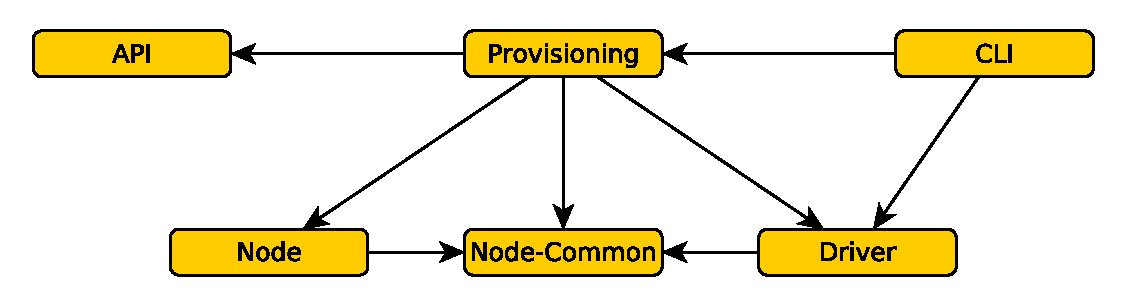
\includegraphics[scale=0.7]{images/module-deps.pdf}
\caption{Clustermeister module dependnecies. The arrows illustrate depends-on relationships. The dependencies are conceptually assigned into two rows. The first row consists of CLI, Provisioning and API. The second row consists of Driver, Node and Node-Common.}
\label{fig:deps}
\end{figure}

\subsection{API}

JPPF offers its own API as ``JPPF client''. Clustermeister uses the JPPF client to connect to the local JPPF driver and to send jobs internally. However, Clustermeister wraps this JPPF client with its own API that simplifies job execution and reduces the configuration to a minimum. To achieve this, Clustermeister offers its own job and task interfaces. However, the Clustermeister API permits access to the JPPF native API, if more control over job execution is desired. Further, it offers a Java \texttt{ExecutorService} that is inherited from the JPPF client API.

The Clustermeister API and its interfaces are designed to reduce configuration as much as possible, but some configuration is still necessary. In section \ref{configuration} the configuration options are discussed in detail.

JPPF Client that connects to local driver
+ custom Job/Task classes, access to native API, ExecutorService
+ Configuration?

interface to distributed infrastructure from user code

\subsection{Provisioning and Deployment}
Most of Clustermeister's functionality is implemented in the provisioning module. This module is responsible to start and manage Clustermeister nodes and make them available to users of the Clustermeister API. In order to provide this functionality, the provisioning module must   

(TODO: check this paragraph)
JPPF is at the core of Clustermeister. JPPF provides a runtime for remote nodes and a server implementation that can run locally. The two target platforms for Clustermeister were Torque/PBS and Amazon EC2, and early tests installing JPPF runtimes on those platforms manually were successful. The goal of Clustermeister, however, was to automate this deployment and provide mechanisms to dynamically add and remove remote nodes to the computation cluster. In the following, properties of those two platforms are discussed.

- local JPPF driver + node deployment code + utilities (dep. resolution, ssh, ...)
- dynamic classloading solved by JPPF
- dep preloading impl. with aether
- SSH impl with jsch
- Amazon with jclouds, parallel
- Torque qsub...
- implements API interfaces
- remote logging
- node management



\subsubsection{lala}

\subsubsection{Torque}

\label{implementation-torque}

Torque offers a generally static infrastructure for deployment. Computations tasks are started from a job submission machine that is accessed via SSH and Torque users have SSH access to this machine.

When accessed via SSH, Torque jobs are submitted with the \texttt{qsub} command. In Clustermeister, the job submission machine is accessed via SSH, then artifacts are uploaded and each node is started as a separate \texttt{qsub} job submission. Depending on how many CPU cores are requested for each job and how many jobs are issued by other participants, these nodes are started immediately or they may be queued. This is one of the difficulties involved with Torque, as node startups cannot be directly controlled.

Another difficulty is network access to nodes. A Torque cluster network is commonly isolated, therefore nodes are allowed to initiate connections, even to resources outside of the local network, but the nodes themselves are not accessible from outside. These constraints lead to difficulties in node management, because the JPPF node management infrastrucure relies on JMX\footnote{http://www.oracle.com/technetwork/java/javase/tech/javamanagement-140525.html} and requires a direct connection to the node. Clustermeister circumvented this problem by extending the JPPF node runtime with management job extensions. These jobs are submitted equally to common computation tasks, but contain meta-data that is handled by the nodes. For example, if a node needs to be shut down, Clustermeister issues a special task and nodes react on it. These special tasks are not dynamic and need to be integrated before the node runtime is deployed. Therefore management tasks cannot be changed or installed while the node is running.

\subsubsection{Amazon}
The Amazon provider component manages Amazon EC2 instances and deploys JPPF nodes on them. The Amazon EC2 service offers many options for customizing and running instances. Clustermeister relies on the jClouds\footnote{http://www.jclouds.org/} library to interact with the EC2 API. It has been chosen because it supports all required features, is well maintained and offers its own API which is not specific to the underlying cloud computation service. This allows to extend Clustermeister with support for other services in the future.

The Amazon provider has been implemented such that it is able to build complex JPPF topologies\footnote{http://www.jppf.org/doc/v3/index.php?title=JPPF\_Overview\#Architecture\_and\_topology} \footnote{http://www.jroller.com/jppf/entry/master\_worker\_or\_p2p\_grid}. This means it can deploy arbitrary numbers of JPPF nodes and servers to any EC2 instance. However bugs in JPPF prevented this functionality to be fully active in Clustermeister. Therefore the provider supports the topology described in section \ref{topology} only

\subsubsection{Utilities}

\begin{description}
 \item[SSH] Both provisioning targets use jsch\footnote{http://www.jcraft.com/jsch/} for SSH access. However, the Amazon target uses jsch via the jclouds API, because jsch is integrated with jclouds. Further, nodes on Amazon instances use a reverse SSH tunnel to connect to the JPPF driver on the local machine.
 \item[Dependency Preloading] In the configuration file, the end-user can configure a pom.xml file or custom entries for dependencies that should be deployed to the node. This is implemented with the aether\footnote{http://www.sonatype.org/aether} library. For more information on how to configure this, see section \ref{appendix-general-configuration}.
 \item[Remote Logging] Logging output from (remote) nodes can be redirected to the local machine. This feature is implemented with log4j remote logging.
\end{description}


\subsection{CLI}

The CLI (command line interface) is a user interface for provisioning and can be seen as a front-end for the provisioning module. The command line interface contains a simple shell that allows to execute commands. The shell itself is implemented with the jline\footnote{http://jline.sourceforge.net/} library, which handles console input and offers features like command auto completion and a history mechanism.

A guide on how to use the command line interface can be found in section \ref{tutorial}.

jlines -> command completion
config loading
user interface for provisioning

\subsection{Node and Driver}
Builds self containing deployable node package
Builds self containing deployable driver package, can be deployed on instances but also used for the local driver

\section{Organisation}

The project duration has been scheduled to three and a half to maximum four months and there has been no pre-existing code base to work from. The project team consisted of two students that worked approximately three days a week on the project. The project definition contained some organizational specifications for the Clustermeister project. Namely that the project shall be licensed under the Apache License, Version 2.0\footnote{http://www.apache.org/licenses/LICENSE-2.0.html}, developed on GitHub\footnote{https://github.com/} and make use of github's issue management and documentation facilities. Therefore Clustermeister is an open source project and all source code and documentation is publicly available at: \url{https://github.com/nethad/clustermeister}.

Given these specifications a number of coarse work items were identified:
\begin{enumerate}
\item \label{wi:spec}Specify the desired system's architecture and functionality (refer to section \ref{architecture} for more information).
\item \label{wi:res}Research and evaluate existing frameworks and libraries for re-use in this project. Particularly frameworks for parallel code execution in distributed JVMs.
\item \label{wi:fam}Familiarize with the desired target computation environments, Amazon Web Services Elastic Compute Cloud (EC2) and TORQUE (PBS).
\item \label{wi:impl}Implementation of the system (refer to section \ref{implementation} for more information).
\item \label{wi:eval}Testing and Evaluation of the solution.
\end{enumerate}

\subsection{Schedule}

The project team estimated the time necessary to spend on each work item and then defined a schedule (see Tab. \ref{tab:schedule}). Work items \ref{wi:res} and \ref{wi:fam} are included in the phase \emph{Evaluation} in the first three weeks. This phase should result in choosing a viable framework for the solution. Next the phase \emph{Implementation 1} follows, which contains the specification and architecture of the solution (work item \ref{wi:spec}) and focuses on implementation of the provisioning module (part of work item \ref{wi:impl}). The provisioning module is a critical centrepiece of the project. In week 10 it the evaluation of the performance of the provisioning module should become a focus (phase \emph{Evaluation 1}, part of work item \ref{wi:eval}). This does not mean that no tests are run before, but that week focuses on identifying critical problems before it is too late to repair them. The phase \emph{Implementation 2} gives opportunity to correct problems and implement the API (work items \
ref{wi:impl}). The last weeks (\emph{Evaluation 2}) should then focus on evaluating the complete system (work item \ref{wi:eval}) and correcting bugs (\ref{wi:impl}). The schedule is not to be interpreted as a definitive work plan in the style of the waterfall model\footnote{http://en.wikipedia.org/wiki/Waterfall\_model}. It associates to each week of the planned project duration the primary type of work that should be performed. For example: In the fifth week the project team will start work on the implementation of the Amazon EC2 provisioning module. The schedule then allows to identify how progress in the project is developing and if the project is on schedule or if action needs to be taken to be able to finish on time. That does not mean that in the fifth week work is restricted to the Amazon EC2 provisioning module, nor that no work is done on the EC2 module in other weeks.

\begin{table}[hptb]
\centering
\begin{tabular}{|l|l|p{7cm}|}
\hline
\textbf{Week} & \textbf{Phase} & \textbf{Major Tasks} \\ \hline
30.1. - 5.2. & Evaluation & JPPF, GridGain, Hazlecast, jClouds \\ \hline
6.2. - 12.2. & Evaluation & Prototyping with JPPF, Amazon EC2, Torque \\ \hline
13.2. - 19.2. & Evaluation & Prototyping Torque, Evaluation Wirr, JPPF Ext. features \\ \hline
20.2. - 26.2. & Implementation 1 & Provisioning: Architecture, API: Architecture \\ \hline
27.2. - 4.3. & Implementation 1 & Provisioning: Amazon \\ \hline
5.3. - 11.3. & Implementation 1 & Provisioning: Amazon \\ \hline
12.3. - 18.3. & Implementation 1 & Provisioning: Torque \\ \hline
19.3. - 25.3. & Implementation 1 & Provisioning: Torque \\ \hline
26.3. - 1.4. & Implementation 1 & Reserved \\ \hline
2.4. - 8.4. & Evaluation 1 & Run first Performance/Scalability Tests \\ \hline
9.4. - 15.4. & Implementation 2 & Implement Lessons Learned from Evaluation \\ \hline
16.4. - 22.4. & Implementation 2 & Implement Lessons Learned from Evaluation \\ \hline
23.4. - 29.4. & Implementation 2 & API \\ \hline
30.4. - 6.5. & Implementation 2 & API \\ \hline
7.5. - 13.5. & Implementation 2 & Reserved \\ \hline
14.5. - 20.5. & Evaluation 2 &  \\ \hline
21.5. - 27.5. & Evaluation 2 &  \\ \hline
28.5. - 3.6. & Evaluation 2 &  \\ \hline
\end{tabular}
\caption{Project Schedule.}
\label{tab:schedule}
\end{table}

\subsection{Working Methodology}

The two students worked on the project in a co-located environment. Since this was a small team, organization was often informally agreed upon. While responsibility for different parts of the system were split (e.g. between Amazon EC2 and Torque modules) they worked as a team, sometimes employing techniques such as code review or pair programming. In general the work methodology followed the ideas of agile software development\footnote{http://en.wikipedia.org/wiki/Agile\_software\_development} and iterative development. When starting work on a scheduled work item, the task was split into numbered \emph{Issues} that captured a confined unit of work (see Fig. \ref{fig:issues}). Issues have been worked on one at a time. This helped with the intention to avoid putting the code base into an inconsistent state because an issue could only be completed when it was properly implemented and tested. While the methodology did not necessarily follow the approach of test driven development\footnote{http://www.agiledata.
org/essays/tdd.html}, great effort was taken to write unit tests for most of the system in order 
to verify functionality in isolation. Additionally a small framework for integration tests has been written to ensure the solutions overall health.

\begin{figure}[hptb]
\centering
\includegraphics[scale=0.7]{images/github-issues.pdf}
\caption{Issue Management with GitHub}
\label{fig:issues}
\end{figure}

\section{Evaluation}
This sections summarizes the performance evaluation done with Clusterermeister. Areas of interest are the provisioning and deployment time (the time needed to make distributed Clustermeister nodes available and load user code on them) and job execution times (how Clustermeister can reduce the time needed to complete a computation job). 

\subsection{Provisioning and Deployment Time}

The time to provision the Clustermeister infrastructure strongly depends on the provisioning provider. When executing code on Clustermeister nodes another critical factor is the time to deploy user code and its dependencies on those nodes. 

\subsubsection{Troque Provisioning}
Torque cluster nodes are provisioned by queuing job requests on the queue management server. At some time the request is granted and a JPPF node is started. Provided the request has a high enough priority, this typically happens very quickly. Therefore the major time needed for provisioning falls to uploading the JPPF node executables and user configured libraries to the queue management server. The time for this depends on network latency, bandwidth and the size of configured libraries. However it is a one time investment only, provided the configuration is not changed and Clustermeister is not updated. Finally the JPPF node launches in about 5-8 seconds. For all these reasons the overall provisioning time is hard to predict but typically lies somewhere between 30 seconds and less than 10 seconds.

\subsubsection{Amazon Provisioning}
Amazon nodes can take significantly longer to be made available. While the same delays apply in respect to upload of binary data and launching a JPPF node, the binary files need to be uploaded to each instance and not only to the queue management server as in the Torque case. But the largest delay falls to the time needed for Amazon to make an EC2 instance available (loading a machine image, booting the machine, and configuring firewall and credentials on it). Creating a new instance and launching a Clustermeister node on it takes about 1 minute and 44 seconds on average (with a maximum measured time of 2:15 and a minimum of 1:30). Of course these numbers depend on the user configuration and network latency and bandwidth as well. On the other hand, launching a Clustermeister node on an already running instance takes merely about 8 seconds. To avoid  this long start up time, the Amazon provider performs node provisioning in parallel for all requested nodes.

\subsubsection{Code Deployment}
When a user executes code on Clustermeister, each class that is not available or out of date in a node's classpath, is loaded over the network from the user's classpath. This happens at runtime, one-by-one as the classes are loaded. Loading large amounts of classes or libraries in this way is very inefficient and may take several minutes. To mitigate this problem, Clustermeister offers the ability to pre-load libraries to nodes at provisioning time. Section \ref{appendix-general-configuration} describes how library pre-loading can be used.

\subsection{Execution Time}

Assessing execution time strongly depends on the nature of the computation task at hand. In the context of Clustermeister we are primarily interested in tasks that can be executed in parallel. This section uses the term \textit{job} to describe a single computation task, such as evaluating a list of numbers if they are primes. A job can then be split into a number of \textit{tasks} that can be executed in parallel (e.g. each number can be checked in parallel, provided there are enough resources). For the purposes of this evaluation two different kind of jobs were evaluated. Namely jobs that consists of a large number of trivial tasks with short execution time. And jobs that consist of a small number of long-running tasks. These two kinds of jobs behave very differently and as will be demonstrated, require different load-balancing (task distribution) algorithm for optimal performance. Clustermeister does not perform any load balancing but allows to configure the load balancing algorithm used by JPPF. The 
available choices are\footnote{http://www.jppf.org/doc/v3/index.php?title=Configuring\_a\_JPPF\_server\#Load-balancing}:

\begin{enumerate}
 \item \textbf{manual}: with this strategy, the user can provide a number of tasks that are executed on each node at most at the same time.
 \item \textbf{autotuned}: this strategy uses an adaptive heuristic algorithm based on the Monte Carlo algorithm.
 \item \textbf{proportional}: an adaptive deterministic algorithm based on the contribution of each node to the overall mean task execution time.
 \item \textbf{rl}: adaptive algorithm based on reinforcement learning.
 \item \textbf{NodeThreads}: each node receives at most n * m tasks, where n is the number of threads the node is configured to use, and m is a user-defined factor. 
\end{enumerate}

In the remainder of this section the data and conclusions obtained from this evaluation are presented.

\subsubsection{Job with many Short-Running Tasks}
\label{short-tasks}

For this evaluation the computation of an image of the Mandelbrot set\footnote{http://en.wikipedia.org/wiki/Mandelbrot\_set} has been chosen. The job creates a task for each row of the image and the task computes an array of color values. The computation of a single task is very fast (fractions of a second) but there are many tasks (600 tasks for an image with resolution 800 x 600). The evaluation was done with the Amazon EC2 provider on \textit{t1.micro} instances\footnote{http://aws.amazon.com/ec2/instance-types/}. The nodes were configured to use only one thread to computation so they could only execute one task at a time. For each run the job was configured to calculate the same part of the image to obtain comparable execution times. 

The first evaluation concentrated on the influence of the load balancing algorithm on execution times. This is not an evaluation of the load balancing algorithms but  an evaluation how much the execution time differs between the worst case and the best case. One part of the execution time measured is network overhead for sending the tasks to the nodes. JPPF can send multiple tasks in batches to nodes. The tasks are then queued on the node for execution but can not be sent to any other node any more. Another strategy is to queue the tasks on the JPPF server and distribute them to nodes as resources become available. To archive this behaviour, the NodeThreads algorithm has been chosen. Because each node has been configured with one thread only, the multiplicator (m) setting for this strategy determines the number of tasks that will be sent to each node in a batch (provided there are enough tasks to satisfy all upper limits).

The working hypothesis was that, assuming all nodes have equal computational resources, for tasks where the \textit{computation time} is much smaller than the \textit{network latency}, the optimal strategy is to distribute all tasks to all available nodes in one batch (see Tab. \ref{tab:mandelbrot-lb}). Contrary, the worst strategy would be to open a dedicated connection for every single task to send it to a node for execution (this equals batches of size 1). In this scenario there is a strong disproportion between network overhead and task computation time in favour of network overhead. The computation time of a task is simply too short to justify paying the overhead of establishing a dedicated connection over the network for every single task. Thus network overhead is expected to be the dominating factor in overall job execution time.

The hypothesis has been tested by running this evaluation on 6 nodes with the NodeThreads load balancing strategy and a multiplicator setting of 100 (best case) and 1 (worst case). The resulting execution times can be seen in Tab. \ref{tab:mandelbrot-lb-res}. It is very obvious that choosing the right load balancing strategy to minimize network latency is very important. The best case scenario is more than 14 times faster than the worst case scenario. And the difference is network overhead.

\begin{table}[h!]
\centering
\begin{tabular}{|c|c|}
\hline
\textbf{Tasks scheduled per node} & \textbf{Job Execution Time [ms]} \\ \hline
100 & 851 \\ \hline
1 & 12156 \\ \hline
\end{tabular}
\caption{Results of running the Mandelbrot set computation on 6 nodes with best case and worst case load balancing settings.}
\label{tab:mandelbrot-lb-res}
\end{table}

The other evaluation concentrated on the influence of number of nodes on execution time. More nodes equal more computation power but also more load balancing and network communication overhead. For this evaluation the load balancing strategy has been manually configured for optimal values under the assumption that each node has has equal resources (see Tab. \ref{tab:mandelbrot-lb}). Fig. \ref{fig:times-mandelbrot} shows the execution times for the Mandelbrot set job for 1 to 6 nodes. As expected the execution time is reduced for each node added. Using 6 nodes instead of 1 node, more than halves the execution time. However the decrease is not linear as the overhead increases with larger number of nodes.

\begin{table}[h!]
\centering
\begin{tabular}{|c|c|}
\hline
\textbf{\# of Nodes} & \textbf{Tasks scheduled per node} \\ \hline
1 & 600 \\ \hline
2 & 300 \\ \hline
3 & 200 \\ \hline
4 & 150 \\ \hline
5 & 120 \\ \hline
6 & 100 \\ \hline
\end{tabular}
\caption{Optimal load balancing settings for the Mandelbrot set evaluation. The goal is to distribute all tasks to all available nodes in one batch.}
\label{tab:mandelbrot-lb}
\end{table}

\begin{figure}[h]
\centering
\includegraphics[scale=0.7]{images/amazon-duration.pdf}
\caption{Execution times for the Madelbrot set calcualtion job.}
\label{fig:times-mandelbrot}
\end{figure}

\subsubsection{Job with few Long-Running Tasks}

\begin{figure}[hptb]
\centering
\includegraphics[scale=0.7]{images/long-running-duration.pdf}
\caption{Long-running tasks}
\label{fig:evaluation-long-running}
\end{figure}

In the simulation with long-running tasks, there were 30 tasks that had a duration of 5 seconds each. In fig. \ref{fig:evaluation-long-running}, the results of the simulation are shown in a chart. The number of nodes were increased from 1 to 6 for each simulation. Each node had one processing thread. In the simulation with 6 nodes, the optimal execution distributes 5 tasks for each node. Each task has a duration of 5 seconds, therefore the optimal execution time is 25 seconds. In the simulation, there was a duration of 25.928 seconds. Hence for long-running tasks, network overhead is neglectable and nodes are always fully utilized.

\subsubsection{Adaptive load balancing algorithms}

JPPF offers a number of adaptive load balancing strategies. These algorithms usually need to execute a number of jobs before they achieve good results. Their task distribution behaviour depends on statistics about a node's past performance and overall execution time. When very similar jobs (in terms of task number/execution time) are submitted repeatedly they often achieve close to optimal performance. However they can easily be thrown off when a job's tasks are very heterogeneous.

Another advantage of adaptive algorithms is that they can automatically tune the load balancing on a per node basis when the participating nodes have very different computation power. Therefore a weak node would receive less tasks than a strong node. This would be complicated or even impossible to achieve manually with the provided configuration options.

Figure \ref{fig:evaluation-learning} shows the job execution times for the Mandelbrot set evaluation (see section \ref{short-tasks}) when using the reinforced learning (rl) and the proportional load balancing strategies.

\begin{figure}[h]
\centering
\includegraphics[scale=0.7]{images/learning-duration.pdf}
\caption{Execution times for the Mandelbrot set job for 10 runs with adaptive load balancing strategies.}
\label{fig:evaluation-learning}
\end{figure}

\subsubsection{Execution Time Conclusions}

The conclusions from this evaluations of execution times is that it is critical to choose the right load balancing strategy depending on the type of computation that is performed. When a task's computation time is much smaller than the network latency, it is important to minimize the task batches sent over the network by choosing an optimal batch size. When the tasks execution time is much larger than the network latency, it is best to not distribute tasks to nodes pre-maturely but instead queue the tasks on the server and send only small batches to nodes to prevent any node from becoming idle for a long time because no tasks are available for scheduling.

Finally, adaptive algorithms can be very good depending on the use case. If a user wants to execute only a single very long running job, adaptive algorithms are a bad idea. It is better to manually tune the load balancing settings. But if many jobs are going to be executed during a session, the adaptive algorithms will learn to perform well. Especially when the available nodes have very different computation power.

\newpage

\appendix

\input{appendix-manual.tex}


\end{document}
